\chapter{Realisierung}
\label{chap:umsetzung}

\section{C-API}
\label{sec:capi_rel}

In folgendem Kapitel wird beschrieben wie die C-API genutzt werden kann, um den Roboter bestimmte Wegpunkte abfahren zu lassen.

\subsection{Beispielanwendung}
\label{sub:capi-problems_rel}

Es konnte eine Anwendung erstellt werden, die den Roboter initialisiert und dann in einer Schleife die Positions-, Geschwindigkeits-und Beschleunigungsdaten sendet. Des weiteren konnte ein Bewegungsprofil errechnet werden, dem der Roboter gefolgt ist.
\\\\
Bevor man Daten vom Roboter abfragen kann, muss eine Verbindung zum Roboter hergestellt werden, ihn mit Strom versorgen und initialisieren lassen. Folgend werden diese Vorgänge beschrieben.\\
Mit dem Befehl \sona{robotinterface\_open()} kann die Verbindung zum Roboter hergestellt werden.
\\\\
Um sicherzugehen, dass die Verbindung offen ist, wird wiederholend in einer Zeitspanne, immer wieder abgefragt, ob der Roboter verbunden ist. Falls dies nicht funktioniert, wird der Vorgang abgebrochen und das Programm sollte beendet werden. Es kommt vor, dass der Roboter beim Starten noch in einem Sicherheitsmodus ist. Wenn dies der Fall ist, muss der Modus abgestellt werden. Dies geht mit der Funktion \sona{robotinterface\_unlock\_security\_stop();}.
\\\\
Auch hier wird zur Sicherheit, der Befehl wiederholt an den Roboter gesandt. Wenn der Roboter dennoch im Sicherheitsmodus bleibt, ist es möglich, dass der Notausschalter am Touch Tablet aktiviert ist.
\\
Nachdem die Verbindung offen ist, muss der Roboter mit Strom versorgt werden. Mit dem Befehl \sona{robotinterface\_power\_on\_robot()} kann das bewerkstelligt werden. Auch hier wird wiederholend gewartet und abgefragt, bis der Roboter hochgefahren ist. Ob der Roboter hochgefahren ist, kann mit der Funktion \sona{robotinterface\_is\_power\_on\_robot()} abgefragt werden.
\\\\
Nun wird der Roboter initialisiert. Er geht nach dem Starten automatisch in den Initialisierungs-Modus. Jedes einzelne Gelenk muss nun so lange in eine Richtung bewegt werden, bis das Gelenk in den normalen Modus übergeht. Um die Gelenke zu bewegen, wird eine Geschwindigkeitsvorgabe an den Roboter gesandt. (siehe Listing \ref{lst:initialize_robot_lst})

\begin{lstlisting}[language=C,caption={Initialisierung der einzelnen Gelenke}, label=lst:initialize_robot_lst,captionpos=b]
puts("Initializing robot");
/// Set zero velocity and acceleration as guard
int j;
for (j=0; j<6; ++j) {
  pva_packet.velocity[j] = 0.0;
  pva_packet.acceleration[j] = 0.0;
}
do {
  ++i;
  robotinterface_read_state_blocking();
  int j;
  for (j=0; j<6; ++j) {
    // initialize_direction is 1 or -1. it determines in which direction die Joint is moving during the initialization
    pva_packet.velocity[j] = ((robotinterface_get_joint_mode(j) == JOINT_INITIALISATION_MODE)) ? (initialize_direction)* 0.1 : 0.0;
   }
  robotinterface_command_velocity(pva_packet.velocity);
  robotinterface_send();
} while (robotinterface_get_robot_mode() == ROBOT_INITIALIZING_MODE && exit_flag == false);
puts(" Done!");
\end{lstlisting}

Nachdem die Initialisierung abgeschlossen ist, muss wie in Listing \ref{lst:robot_control_loop} eine Schleife mit der vorgegebenen Struktur durchlaufen werden, bis das Programm beendet, oder die Verbindung zum Roboter geschlossen werden soll. Wenn dies nicht so gehandhabt wird, geht der Roboter automatisch in den Sicherheitsstopp, da nicht innerhalb von acht Millisekunden Nachrichten an den Roboter gesendet wurden.
\\\\
Innerhalb der beiden Befehle \sona{robotinterface\_read\_state\_blocking()} und \sona{robotinterface\_send()} kann nun eine Interpolation berechnet werden und die Vorgaben für Position, Geschwindigkeit und Beschleunigung an den Roboter gesandt werden(siehe Listing \ref{lst:interpolate}).

\begin{lstlisting}[language=C,caption={Interpolation eines berechneten Wegs}, label=lst:interpolate,captionpos=b]
// loop through interpolation length  
for(i=0; i < move_pva_packet.interpolations+1; i++){
  robotinterface_read_state_blocking();

  // abort interpolation if Robot is in securitystop mode
  if(robotinterface_is_security_stopped()) {
      robotinterface_get_actual_current(currents_actual);
      robotinterface_command_empty_command();
      robotinterface_send();
      break;
  }

  // get current time of interpolation 
  move_pva_packet.point_in_time= (double) i * T_IPO;

  // interpolate with sinoide profile and write result in variable move_pva_packet
  interpolation_sin_ptp(&move_pva_packet);

  // write the triple to robot
  robotinterface_command_position_velocity_acceleration(move_pva_packet.pva.position,
                                                        move_pva_packet.pva.velocity,
                                                        move_pva_packet.pva.acceleration);
  // send command to robot
  robotinterface_send();
}
\end{lstlisting}

\subsection{Bewegungsprofil berechnen und interpolieren}
\label{sub:profile_and_interpolation_rel}

Ein Bewegungsprofil besteht aus 3 Phasen: Beschleunigungs-, Konstantfahrt-und Bremsphase.
Die Formeln für die Berechnung sind dem Buch ``Industrieroboter: Methoden der Steuerung und Regelung'' \cite{WW-2013} entnommen.
\\
Eine sanfte Beschleunigung schont die Robotergelenke. Dies wird auch Sinoidenprofil genannt. Die Formeln in der Lektüre können einfach übernommen und müssen nur ausprogrammiert werden. In der Dokumentation ist die Interpolation und Berechnung für eine PTP-und Linear-Bahn
genau beschrieben.
\\\\
Um die Berechnung des Profils zu testen, kann simuliert interpoliert werden und die einzelnen Angaben in den Interpolationsschritten geloggt werden. Nachher werden die geloggten Daten in Matlab\footnote{``MATLAB® ist eine höhere Programmiersprache und interaktive Umgebung für numerische Berechnungen, Visualisierung und Programmierung. MATLAB dient zur Datenanalyse, Algorithmen-Entwicklung und zur Erstellung von Modellen und Anwendungen.''\cite{MATLAB-2014}} geplottet.
Folgend sind die Profile der Positions-, Beschleunigungs-und Geschwindigkeitswerte für eine PTP-Bahn geplottet.

\begin{figure}[H]
  \centering
    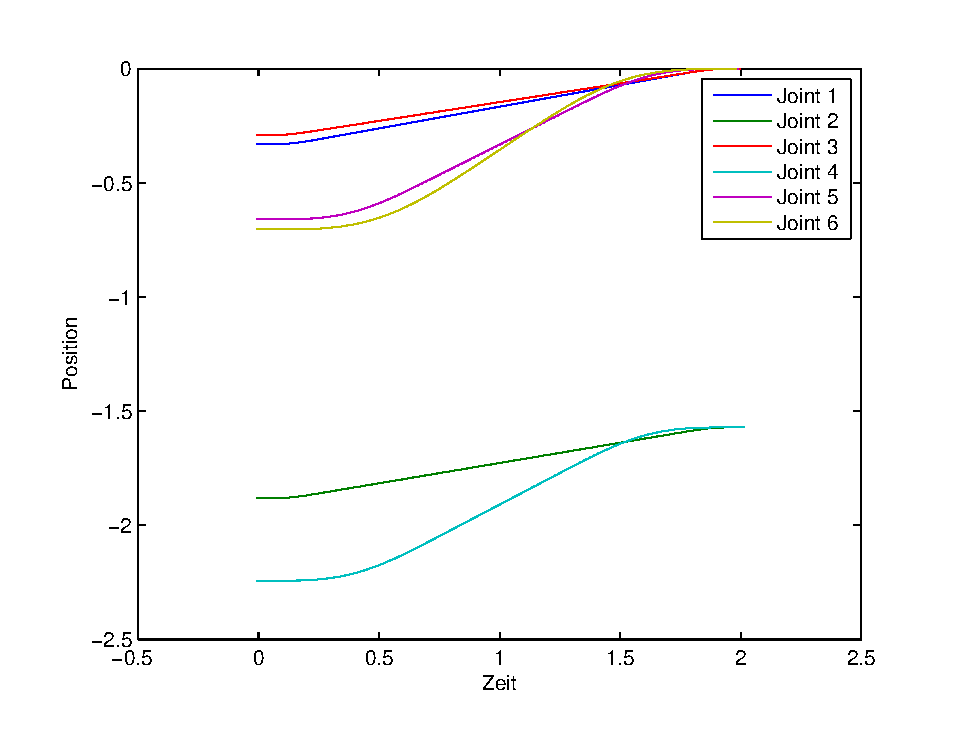
\includegraphics[width=0.8\textwidth]{pic/position_profile.eps}
      \caption[Positionsprofil einer PTP-Bahn in Matlab gepplotet]{Die Abbildung zeigt das Positionsprofil einer PTP-Bahn mit allen Gelenken. Position ist angegeben in Radiant.}
      \label{fig:position_ptp_profile}
\end{figure}

\begin{figure}[H]
  \centering
    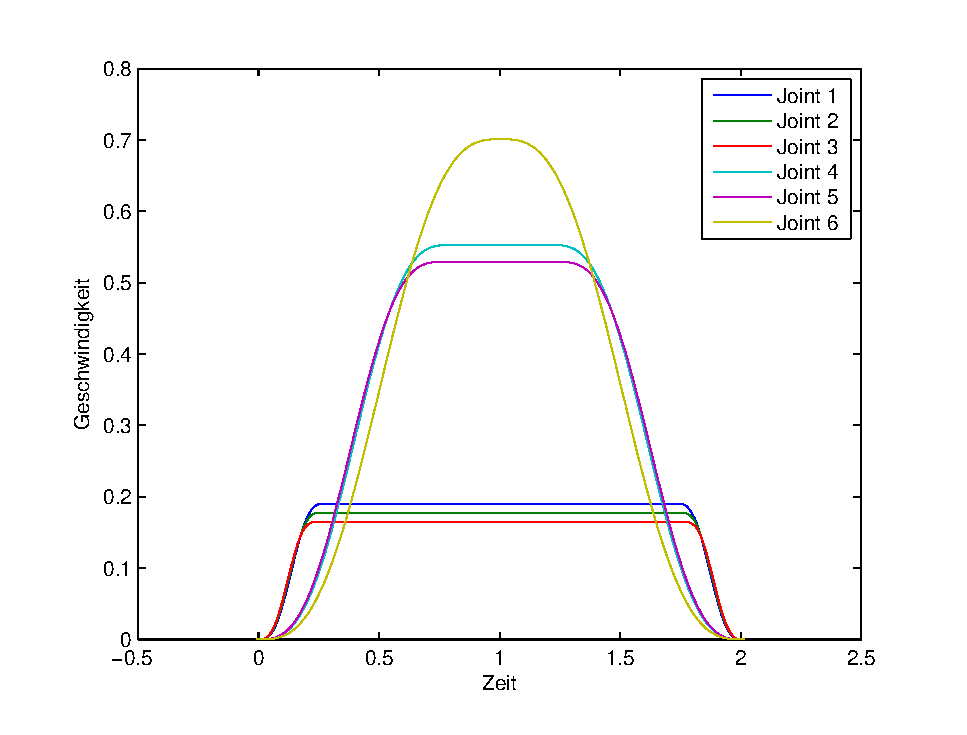
\includegraphics[width=0.8\textwidth]{pic/velocity_profile.eps}
      \caption[Geschwindigkeitsprofil einer PTP-Bahn in Matlab gepplotet]{Die Abbildung zeigt das Geschwindigkeitsprofil einer PTP-Bahn mit allen Gelenken. Die Geschwindigkeit ist angegeben in Radiant/Sekunde.}
      \label{fig:velocity_ptp_profile}
\end{figure}

\begin{figure}[H]
  \centering
    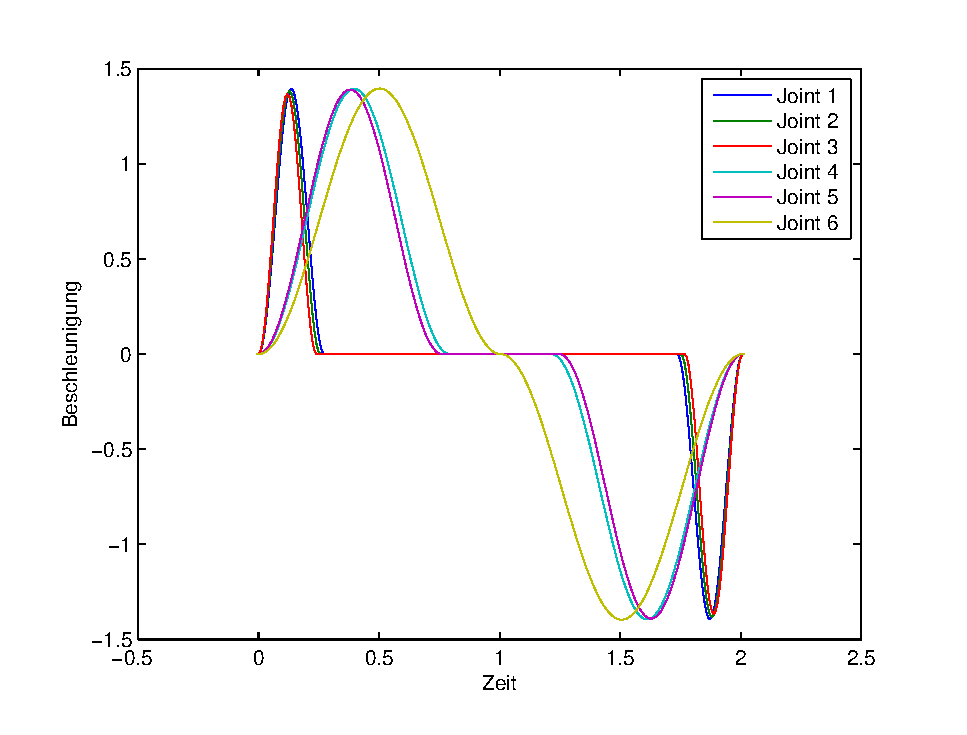
\includegraphics[width=0.8\textwidth]{pic/acceleration_profile.eps}
      \caption[Beschleunigungsprofil einer PTP-Bahn in Matlab geplottet]{Die Abbildung zeigt das Beschleunigungsprofil einer PTP-Bahn mit allen Gelenken. Die Beschleunigung ist angegeben in Radiant/Sekunde²}
      \label{fig:acceleration_ptp_profile}
\end{figure}

\subsection{Aufgetretene Probleme}
\label{sub:capi-problems_rel}

Der Roboter geht ab einem bestimmten Winkel in den Sicherheitsstopp. Die Abweichung der Position wird zu groß. Dies kann analysiert werden, wenn man sich den Durchschnitt der Soll-und Ist-Werte der Position ansieht (siehe Abbildung \ref{fig:position_join1}). Es ist deutlich zu erkennen, dass die Abweichung beim 2. Gelenk steigt. Die Motorleistung reicht anscheinend nicht aus, um über die Schwelle der Reibungskräfte und die Erdanziehung zu kommen. Zu sehen ist in Abbildung \ref{fig:joint_1_position_capi}, dass für die Stromstärke ein Offset mitberechnet wird. Vergleicht man die Werte, die bei derselben Bewegung von Polyscope berechnet werden (siehe Abbildung \ref{fig:current_profile_joint1_rci}), sieht man eine höhere Stromstärke bei der Polyscope Software, bei der die Bewegung ohne Probleme funktioniert.
\\
\begin{figure}[H]
  \centering
    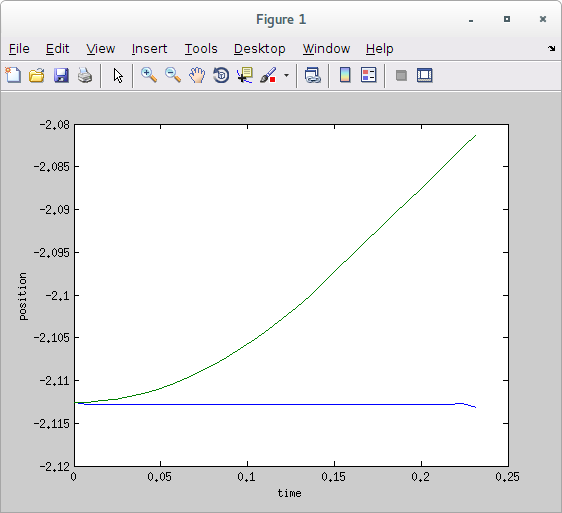
\includegraphics[width=0.6\textwidth]{pic/joint1_position_capi.png}
      \caption[Soll-und Ist-Werte der Position]{Abbildung zeigt die Soll-und Ist-Werte der Position bis zum Sicherheitsstop des Roboters}
      \label{fig:position_join1}
\end{figure}

Mit der C-API ist es nicht möglich, selbst den Wert der Stromstärke vorzugeben, deswegen sind die Soll-Werte bei der Polyscope Software und der eigenen Anwendung mit der C-API etwas verschieden.
\\
Bei dem 2. Gelenk ist auch zu beobachten, dass dieses nicht rechtzeitig anhält, wenn der Notausschalter betätigt wird. Bei einem solchen Versuch ist der Roboter zu spät angehalten. Deswegen ist auch eventuell von einem Hardwaredefekt auzugehen.

\begin{figure}[H]
  \centering
    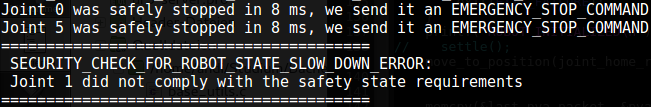
\includegraphics[width=0.8\textwidth]{pic/emergency_stop_capi.png}
      \caption[Warnungsausgabe für 2. Gelenk nach Notausschalter]{Abbildung zeigt eine Warnung die von der C-\ac{API} ausging, weil das 2.Gelenk nicht rechtzeitig nach einem Notaus angehalten hat}
      \label{fig:acceleration_ptp_profile}
\end{figure}
\newpage
\section{Polyscope}
\label{sec:Polyscope_rel}

\subsection{Programmierung}
\label{sub:programmierung_polyscope_rel}

Die Programmierung findet meist nur auf dem Touch Tablet statt. Ein neues Programm fängt mit einem leeren Ereignisbaum an. Es können per Toucheingabe alle möglichen Funktionen, die die Script Sprache bietet, dem Ereignisbaum hinzugefügt werden. Wenn das Programm abläuft, werden von der Wurzel an die Befehle abgearbeitet.
Wie in Abbildung \ref{fig:programm_in_polyscope} zu sehen ist, ist die Ansicht des Programmbaumes sehr unübersichtlich.

\begin{figure}[H]
  \centering
    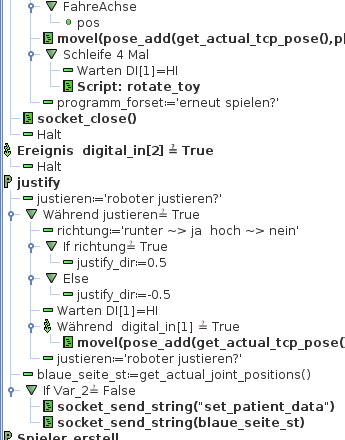
\includegraphics[width=0.5\textwidth]{pic/polyscope_program_tree.png}
      \caption[Programm Baum in Polyscope]{Ein Ausschnitt aus einem Programm Baum in Polyscope}
      \label{fig:programm_in_polyscope}
\end{figure}

Es ist möglich, andere Script Dateien in das Programm einzufügen. Dazu gibt es das Feld \sona{Script}. Das Script-Programm muss sich auf dem Linux-Rechner befinden. Man muss daher das Script Programm auf einem anderen Rechner programmieren und bei jeder Änderung auf den Linux-Rechner des Roboters senden. Mit dieser Möglichtkeit könnten Programmabschnitte ausgelagert werden. Es ist aber nicht ersichtlich, welche Script Dateien benutzt werden.\\
Alternativ zum Touch Tablet, könnte der X-Server von dem Linux-Rechner auf einen anderen Rechner umgeleitet werden, um dort mit dem Programm per Maus und Tastatur zu arbeiten. Dies wurde aber noch nicht getestet und es könnte zu Verzögerungen beim Ausführen kommen.
\\
Eine andere Möglichkeit, ein Programm unter Polyscope zu programmieren, gibt es nicht.

\subsection{Benutzer-Interaktion}
\label{user_interaktion_polyscope_rel}

Die Möglichkeiten zur Interaktion mit dem Benutzer sind sehr begrenzt. Die Software und die URScript Sprache lassen es zu, dass auf dem Touch Tablet Popups auftauchen. Wenn man mit dem Benutzer interagieren will, gibt es mehrere Arten dieser Popups.
Als Nachricht, ja/nein Fragen, oder Text abfragen. Der Benutzer kann dann mit einem Text antworten oder klickt auf einen Ja-bzw. Nein-Button. In Abbildung \ref{fig:polyscope_popup} ist als Beispiel eine Nachricht und ein Ja/Nein Popup zu sehen.

\begin{figure}[H]
  \centering
    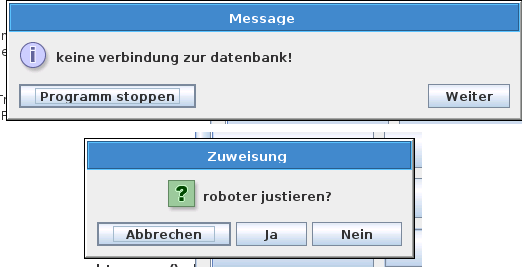
\includegraphics[width=0.8\textwidth]{pic/popup_question.png}
      \caption[Popup in Polyscope]{Abbildung zeigt zwei verschiedene Arten von Popups in Polyscope}
      \label{fig:polyscope_popup}
\end{figure}

Kompliziertere Menüs sind mit dieser Methode nicht möglich. Wenn ein Programm erstellt werden soll, bei dem der Benutzer viele Eingaben machen muss, lässt sich das mit Polyscope nur sehr schwer realisieren.

\subsection{Test und Fehlersuche im Programm}
\label{debuggin_polyscope_rel}

Bevor Polyscope ein Programm ablaufen lässt, wird das Script auf die richtige Syntax geprüft. Sollte ein Fehler vorhanden sein, wird dies beim Start als Popup angezeigt. Fehler, die in Abschnitten mit Touch hinzugefügt wurden, können jedoch nicht lokalisiert werden. Nur in extra eingefügtem Script Code kann grob lokalisiert werden, welcher Fehler aufgetreten ist, weil dieser Teil extra geprüft wird.
\\\\
Da das Programm mit dem Touch Tablet ausgeführt werden kann, kann man während der Programmierung das Programm kurz ablaufen lassen um zu Testen. So kann sehr schnell getestet werden ob die gewünschten Einstellungen dem Ergebnis entsprechen. Bei großen Programmen mit vielen Benutzeranfragen, kann dies jedoch viel Zeit in Anspruch nehmen. Es muss von einem Benutzer bei jeder Anfrage eines Popups von Hand geantwortet werden.

\subsection{Aufwand der Programmierung}
\label{polyscope_aufwand}

Kleine Programme in Polyscope sind schnell geschrieben. Mit dem Touch Tablet kann rapide eine kleine Kontrollstruktur aufgebaut werden. Das Tablet hat jedoch große Nachteile. Wie in Abbildung \ref{fig:programm_in_polyscope} zu sehen ist der Bereich für den Ereignisbaum äußerst klein. Wenn ein Programm nun z. B. 500 Befehle enthält, ist es nicht möglich den Überblick zu behalten. Außerdem ist es ziemlich aufwändig, zwischen bestimmten Bereichen hin und her zu wechseln, da das Touch Tablet nicht genau ist. Es ist möglich, größere Bereiche auf Scirpt Dateien auszulagern, um diese dann im \ac{URP} zu verwenden. Das erlaubt die Wiederverwendung von Code. Mit dem Touch Tablet ist es jedoch nicht angenehm, diese zu programmieren und anzupassen.

\subsection{\ac{TCP/IP} Server mit Datenbank zum dauerhaften Speichern der Daten}
\label{tcp_datentank_sicherung_rel}

Um mit Polyscope und URScript erhobene Daten zu speichern, wurde ein kleiner \ac{TCP/IP} Server geschrieben, der eine Verbindung zulässt und Daten in einer Datenbank speichert. Die Daten sind objektorientiert, und werden von dem Server erstellt.
In Polyscope und URScript gibt es keine Objektorientierung, deshalb muss dort alles nacheinander abgefragt werden.
Ein Beispiel einer \ac{TCP/IP} Servers ist im Anhang aufgeführt (siehe \ref{save_data_tcp_code_gru}).

\section{URScript}
\label{sec:ur_script_rel}

Die URScript Sprache ist sehr stark an Python gelehnt.
Das Manual von Univeral Robots umfasst alle nötigen Funktionen, um komplexe Aufgaben zu erfüllen.
Um Daten persistent zu speichern, muss wie in Polyscope eine Socket-Verbindung zu einer zweiten Anwendung aufgebaut werden, die die Daten speichert (siehe \ref{tcp_datentank_sicherung_rel})

\subsection{Laden des Scripts auf den Controller}
\label{load_script_rel}

Das Script kann nicht direkt auf dem Rechner über die Polyscope Software ausgeführt werden. Um ein selbst geschriebenes Programm in URScript auszuführen, ist es von nöten, sich mit der Secondary Schnittstelle des URControllers \ref{urcontrol_spi_gru} per \ac{TCP/IP} zu verbinden und dann die einzelnen Zeilen der Script Datei an den Controller zu senden.
\\\\
Es ist möglich, einzelne Befehle oder ein großes Programm auszuführen. Um einzelne Befehle auszuführen, werden diese nacheinander versendet.
Ein ganzes Programm wird versendet, indem, wie in Listing \ref{lst:urscipt_program_lst} gezeigt, eine Funktion die ganzen Befehle umschließt. Der Controller führt diese Funktion aus, sobald diese mit dem ``end'' der Funktion abgeschlossen ist.
Zu beachten ist noch, dass der URController am Ende jeden Befehls oder Programms einen Zeilenumbruch erwartet.

\begin{lstlisting}[caption={Kleines Beispielprogramm in URScript}, label=lst:urscipt_program_lst ,captionpos=b] 
def myProg():
	popup("hello world","test", False, False)
	set_digital_out(1, True)
	movej([0.23,1.23,0.343,0.34.0.0,0.0],a=0.5,v=0.3)
end
\end{lstlisting}

\subsection{Programmierung}
\label{programmierung_ur_script_rel}

Programmiert werden kann das Script mit allen vorhandenen Textverarbeitungsprogrammen. Vorteilhaft ist es, wenn das Programm Syntax Highlighting\footnote{Zur Verbesserung der Lesbarkeit und der Übersicht, wird in einem Textverarbeitungsprogramm der Programmcode unterschiedlich dargestellt. Meist mit unterschiedlichen Farbwerten. Der Entwickler sieht mit einem Blick, ob er es mit Textvariablen oder Zahlenwerten zu tun hat.} für Python beherrscht. Da URScript ja sehr stark an Python angelehnt ist, trägt dieses Verfahren zu einem besseren Überblick bei.
\\\\
Die Sprache bietet keine Möglichkeiten, Kommentare zu nutzen, was aber sehr wichtig ist, wenn ein Programm wächst und mehrere Programmierer am Projekt beteiligt sind. Es ist wichtig für die Verständlichkeit. Deshalb wurde dafür in dem Programm, welches das URScript liest und an die Schnittstelle sendet, ein Pre-Prozessor eingebaut. Die Script Datei wird nach Kommentaren durchsucht und schneidet diese vor dem Senden heraus. (siehe \ref{lst:urscipt_comment_lst}).

\begin{lstlisting}[caption={Beispiel-Kommentare vor und nach dem Pre-Prozessor}, label=lst:urscipt_comment_lst ,captionpos=b]
  def testprog():
    # mit # wird ein Kommentar angefangen
    movej([0.23,1.23,0.343,0.34.0.0,0.0],a=0.5,v=0.3) # Bewegung auf Achs Ebene zur Startposition
  end

  wird zu 

  def testprog():
    movej([0.23,1.23,0.343,0.34.0.0,0.0],a=0.5,v=0.3)
  end

\end{lstlisting}

\subsection{Test und Fehlersuche im Programm}
\label{ur_script_debuggen}

Nach dem Senden des Programms an den URController ist die einzige Möglichkeit, zu sehen ob das Programm Fehler enthält, wenn der Controller ein entsprechendes Bit setzt, das in den Datenpaketen von der Secondary Schnittstelle gesendet wird. Über dieses ``Programm läuft'' Bit, kann man sehen ob ein Programm läuft oder nicht.
\\
Wenn das Script Programm nicht abläuft, erhält man keinerlei Fehlermeldungen. Um Fehler auszuschließen, muss also der Bereich isoliert werden, in dem der Fehler vorkommt. Das geht meist nur in einem aufwändigem Ausschlussverfahren, bei dem immer wieder Script Code entfernt wird.

\subsection{Benutzer Interaktion}
\label{ur_script_user_interaction}

Das Manual für URScript nennt nur die Popup-Funktion, um dem Anwender eine Nachricht zu geben. Andere Möglichkeiten zur Interaktion sind im Manual nicht angegeben. Jedoch bietet Polyscope auch über verschiedene Popup-Arten Möglichkeiten zur Interaktion. Diese Popups gibt es auch für URScript. Die Befehle können aus dem von Polyscope erzeugtem URScript Code von \ac{URP}s eingesehen werden. Somit bestehen genau die gleichen Möglichkeiten wie bei Polyscope.

\subsection{Aufwand der Programmierung}
\label{ur_script_aufwand}

Im Gegensatz zur Polyscope Software, kann mit einem Textverarbeitungsprogramm schnell mit guter Übersicht ein größeres, komplexeres Programm erstellt werden. Es können problemlos mit dem Pre-Prozessor Kommentare eingefügt werden und der Code ist im späteren Fall leichter verständlich für neue Programmierer. Da schwer Fehler zu entdecken sind und deswegen häufig das Programm manuell getestet werden muss, ist dennoch bei umfassenden Anwendungen ein größerer zeitlicher Aufwand von Nöten.

\section{Anwendung mit Adapter zu URScript}
\label{sec:script_hoerherer_schicht_rel}

Im folgenden Kapitel wird das Anwendungsbeispiel in Python entwickelt. Um zu zeigen, wie die Benutzerinteraktion mit einem eigenen Adapter gestaltet werden kann, wurde hierfür die Software Bibliothek \sona{TKinter}\footnote{Mehr Informationen über TKinter unter folgender Website: \url{https://wiki.python.org/moin/TkInter}}, mit der man schnell eine \ac{GUI} entwickeln kann. Die Interaktion erfolgt durch Buttons, die dann über den Adapter Befehle an den Roboter sendet.

\subsection{Adapter zur Secondary Schnittstelle}
\label{beschreibung_script_hoeher_schicht}

Die Scriptbefehle zur Secondary Schnittstelle werden als Text übergeben. Der Adapter wird in Form einer Klasse geschrieben, die die einzelnen Script Befehle in Funktionen mitliefert(siehe Listing \ref{lst:secondary_interface_scriptfunctions}).

\begin{lstlisting}[caption={Ausschnitt zeigt Funktionen, die Scriptbefehle in der Adapter-Klasse umsetzt}, label=lst:secondary_interface_scriptfunctions ,captionpos=b]

# moveJ moves the Robot with joint coordinates
# positions should include the target joint positions
def movej(self, positions=None, a_max=None, v_max=None):
    if positions is None:
        positions= self.get_joint_positions()
    if a_max is None:
        a_max=math.radians(40)
    if v_max is None:
        v_max=math.radians(60)
    message="""movej(%s,a=%f,v=%f)
    """%(positions,a_max,v_max)
    print message
    self.start_program(message)

# movel moves the Robot Linear in kartesian coordinates
# positions should contain the target tcp positions
def movel(self, positions=None, a_max=None, v_max=None):
    if positions is None:
        positions= self.get_tcp_positions()
    if a_max is None:
        a_max=math.radians(40)
    if v_max is None:
        v_max=math.radians(60)
    message="""movel(p%s,a=%f,v=%f)
    """%(positions, a_max, v_max)
    print message
    self.start_program(message)
\end{lstlisting}

Diese Klasse öffnet zwei Verbindungen zur Secondary Schnittstelle. Eine zum Empfangen der Datenpakete und eine zum Senden der URScript Befehle. Der Adapter besitzt eine Queue\footnote{Eine Warteschlange, ähnlich wie bei einem Supermarkt. Die Elemente in einer Queue werden nacheinander abgearbeitet.}, um die Befehle nacheinander zur Secondary Schnittstelle zu senden. Da Befehle eventuell viel Zeit benötigen, um ausgeführt zu werden, wird gewartet, bis der Befehl abgearbeitet oder abgebrochen wurde. Erst dann wird in der Queue der nächste Befehl an die Schnittstelle gesendet.

\begin{lstlisting}[caption={Ausschnitt zeigt die Abarbeitung der Queue}, label=lst:adapter_queue ,captionpos=b] 
while self.__run_flag:
    DequePrograms.lock.acquire()
    if(len(self.s_interface.program_queue) > 0):
        # print("message queue contains messsages %d" % len(self.s_interface.program_queue))
        message=self.s_interface.program_queue.popleft()
    else:
        message=None
    DequePrograms.lock.release()
    if(message is not None):
        SecondSendInterface.send_lock.acquire()
        self.s_interface.send_messages_queue.append(message)
        SecondSendInterface.send_lock.release()

        //blocks the thread until URScript finishes
        self.s_interface.block_program()
    time.sleep(0.2)
return 0
\end{lstlisting}

In einer Anwendung kann nun diese Klasse benutzt werden, um den Roboter zu steuern.
Der Aufwand für ein Programm ist mit einer eigenen API anfangs deutlich höher als die URScript-Sprache direkt zu nutzen. Es muss erst ein Adapter geschrieben und getestet werden, bevor die eigentliche Anwendung geschrieben werden kann. 

\subsection{Programmierung mit Adapter}
\label{programmierung_mit_hoerherer_schicht}

Sobald der Adapter in einer etablierten Programmiersprache programmiert ist und Fehler in diesem so gut wie ausgeschlossen sind, kann nun mit normalen Softwareentwicklungstechniken leicht ein Programm geschrieben werden. In dieser Arbeit wurde Python gewählt. Python bietet viele Bibliotheken und Design Patterns, die das Programmieren vereinfachen. Es können Entwicklungswerkzeuge benutzt werden, um einen guten Überblick über das Programm zu behalten.

\subsection{Benutzer-Interaktion}
\label{user_interaktion_mit_hoerherer_schicht}

Eine etablierte Programmiersprache bietet natürlich verschiedene Bibliotheken und Möglichkeiten, ein interaktives und leicht verständliches Interface zu erstellen. Man ist in der Lage, übersichtliche Formulare zu erstellen und Informationen vom Anwender zu erfassen. Abbildung \ref{fig:hda_urcontrol_gui} zeigt ein Interface, mit dem der Roboter primitiv in alle Richtungen gesteuert werden kann.

\begin{figure}[H]
  \centering
    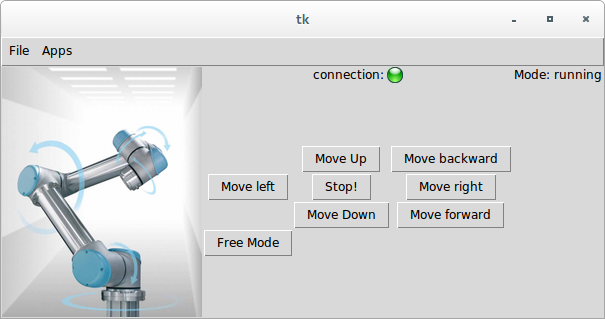
\includegraphics[width=0.8\textwidth]{pic/hda_urcontrol_gui.png}
      \caption[Selbsterstelltes GUI zur Steuerung des UR5 Roboters]{Startfenster des selbst erstellten GUIs zur Steuerung des UR5 Roboters. Der Roboter lässt sich in alle Richtungen linear bewegen.}
      \label{fig:hda_urcontrol_gui}
\end{figure}

\subsection{Test und Fehlersuche im Programm}
\label{debuggen_mit_hoeherer schicht}

Nach Ausschluss der Fehler im Adapter, ist es möglich Unittests\footnote{Unittests erlauben es einzelne Komponenten/Module in einem Programm zu Testen} für das Programm zu benutzen. Die Schnittstelle zum Roboter wird hier durch einen sogenannten Mock\footnote{Ein Platzhalter für Software-Objekte. Wird benutzt, um Software zu testen, bei der ein Teil der Software noch nicht existiert oder ausgeschlossen werden soll.} erstetzt. Dadurch kann auch offline getestet werden. Fehler werden in den etablierten Programmiersprachen so einfach gefunden und lokalisiert. In etablierten Programmiersprachen, sei es eine Sprache die mit einem Interpreter arbeitet oder vorher kompiliert wird, wird vor der Ausführung die Syntax getestet. Deshalb können auch Syntaxfehler im Gegensatz zur URScript-Sprache lokalisiert werden.

\subsection{Aufwand der Programmierung}
\label{eigene_api_aufwand}

Der Aufwand für ein Programm ist mit einer eigenen API anfangs deutlich höher gegenüber den anderen Methoden. Es muss erst ein Adapter geschrieben und getestet werden, bevor die eigentliche Anwendung geschrieben werden kann. 
Nach dieser Hürde, lassen sich jedoch unkompliziert Programme erstellen, die auf den Adapter zugreifen, um den Roboter zu steuern.